\section{Results}\label{sec:results}

\begin{table}[t]
\caption{Accuracy (\%) by condition and cross-repository F1. Tokens: prompt tokens per issue.}\label{tab:acc}
\small
\begin{tabular}{lrrrr}
\toprule
Approach & NLBSE'24 & 2025--26 & New repo & Tokens \\
\midrule
TF-IDF + LR & 75.5 & 66.3 & 60.4 & -- \\
Embedding + LR & 69.3 & 68.5 & 57.5 & -- \\
LLM zero-shot & 68.5 & 71.2 & 68.4 & 0.4k \\
LLM few-shot & 70.9 & 75.3 & 68.0 & 1.1k \\
\midrule
\multicolumn{5}{l}{\emph{Cross-repository F1 (NLBSE ranking metric)}} \\
TF-IDF + LR & 0.754 & 0.583 & 0.592 & \\
Embedding + LR & 0.691 & 0.630 & 0.561 & \\
LLM zero-shot & 0.663 & 0.650 & 0.661 & \\
LLM few-shot & 0.694 & 0.682 & 0.657 & \\
\bottomrule
\end{tabular}

\end{table}

\subsection{RQ1: Accuracy in and out of distribution}
Table~\ref{tab:acc}. In distribution, TF-IDF with logistic regression, trained on only 1{,}005
labeled issues, is the most accurate approach (76.2\%, 95\% CI [74.0, 78.3]); the few-shot LLM reaches
70.9\% [68.6, 73.3] and zero-shot 68.5\%. Out of distribution the order reverses. On 2025--26 issues
TF-IDF drops to 67.5\% and its cross-repository F1 from 0.760 to 0.584, while the few-shot LLM rises to
75.3\%. On a new repository TF-IDF and the embedding classifier fall to 60.3\% and 58.8\%; the LLMs
lose at most 3 points (68.0\%, 68.4\%). The classical models learn repository- and period-specific
vocabulary; the LLM relies on general knowledge of what bugs, features and questions look like.

The 2025--26 issues also serve as a leakage control: they postdate the model's training data, and the
LLM is \emph{more} accurate on them than on the 2016--2023 benchmark, so we see no sign that benchmark
contamination inflates LLM results here. The fresh data show a different kind of drift instead:
label usage. React, for example, labeled 200 bugs but only 9 feature requests and 5 questions in
2025--26, since it now routes questions elsewhere, so a labeler tuned to the benchmark's balanced
classes faces a very different prior.

\begin{figure*}[t]
\centering
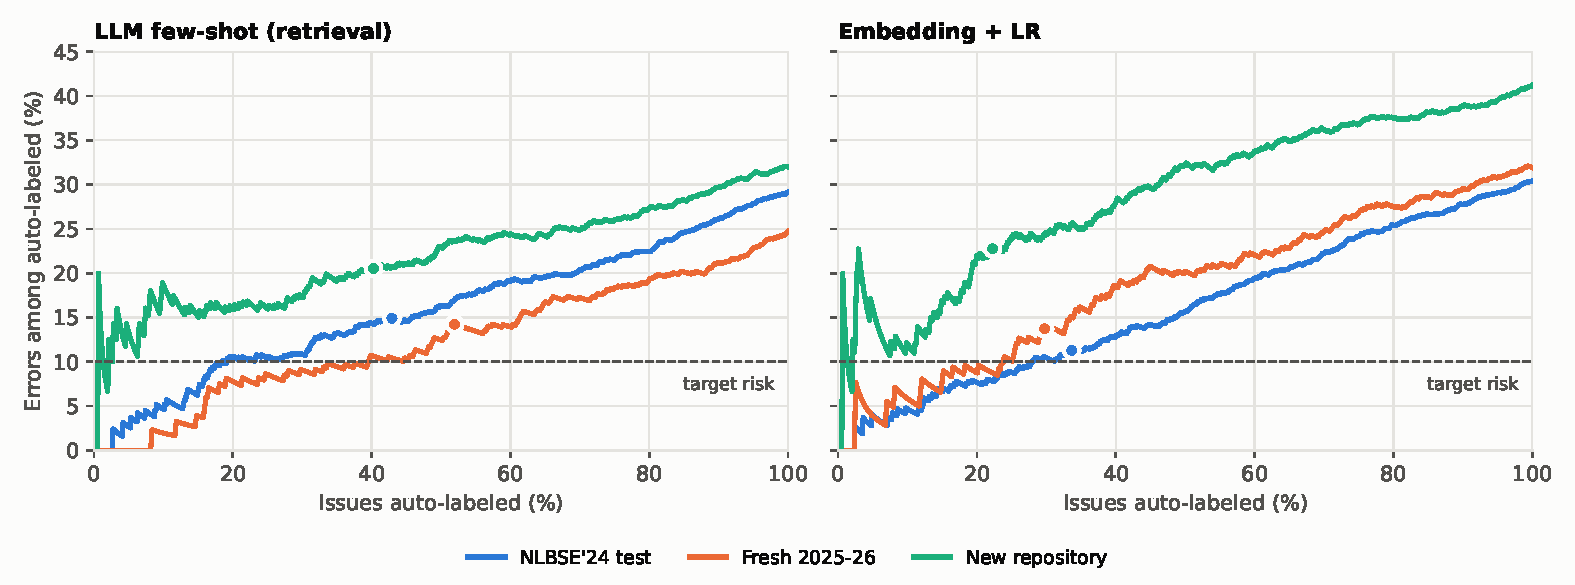
\includegraphics[width=0.92\textwidth]{risk_coverage.pdf}
\caption{Risk--coverage curves: error among the most confident issues as more are auto-labeled.
Dots: the naive threshold calibrated for 10\% error. The dashed line is the target.}\label{fig:rc}
\end{figure*}

\begin{table*}[t]
\caption{Selective automation: coverage / risk (\%), i.e., share auto-labeled / errors among them.
Target risk: 10\%. All thresholds are set on the calibration split.}\label{tab:sel}
\small
\begin{tabular}{llrrr}
\toprule
Approach & Policy & NLBSE'24 & 2025--26 & New repo \\
\midrule
TF-IDF + LR & auto-all & 100.0 / 23.8 & 100.0 / 32.5 & 100.0 / 39.7 \\
 & naive threshold & 54.9 / 12.5 & 48.8 / 19.1 & 33.5 / 26.3 \\
 & risk-controlled & 15.6 / 4.3 & 12.5 / 9.4 & 1.5 / 18.2 \\
 & conformal & 61.9 / 14.5 & 60.7 / 23.7 & 46.5 / 28.9 \\
\midrule
Embedding + LR & auto-all & 100.0 / 30.4 & 100.0 / 31.9 & 100.0 / 41.2 \\
 & naive threshold & 33.7 / 11.3 & 29.8 / 13.7 & 22.3 / 22.8 \\
 & risk-controlled & 13.5 / 5.9 & 11.5 / 5.1 & 8.0 / 11.7 \\
 & conformal & 47.7 / 15.7 & 44.7 / 18.3 & 38.5 / 28.7 \\
\midrule
LLM zero-shot & auto-all & 100.0 / 31.5 & 100.0 / 28.8 & 100.0 / 31.6 \\
 & naive threshold & 13.1 / 12.2 & 24.9 / 7.8 & 10.9 / 14.6 \\
 & risk-controlled & 0.0 / -- & 0.0 / -- & 0.0 / -- \\
 & conformal & 29.5 / 17.8 & 39.3 / 11.4 & 27.1 / 17.2 \\
\midrule
LLM few-shot & auto-all & 100.0 / 29.1 & 100.0 / 24.7 & 100.0 / 32.0 \\
 & naive threshold & 42.9 / 14.9 & 51.9 / 14.2 & 40.3 / 20.5 \\
 & risk-controlled & 6.9 / 3.9 & 8.0 / 0.0 & 1.2 / 11.1 \\
 & conformal & 52.8 / 17.9 & 59.5 / 16.3 & 50.5 / 22.7 \\
\midrule
LLM few-shot + Emb. & agreement & 67.0 / 17.8 & 71.4 / 17.7 & 63.6 / 26.4 \\
\bottomrule
\end{tabular}

\end{table*}

\subsection{RQ2: Does calibrated deferral keep its promise?}
Raw LLM label probabilities are almost always 0 or 1; temperature scaling on the calibration split
needs $T{=}7.6$ (few-shot) and $T{=}10.1$ (zero-shot) and lowers expected calibration error from
0.23--0.30 to 0.05--0.08. The classical models are underconfident ($T{\approx}0.6$).

Table~\ref{tab:sel} and Figure~\ref{fig:rc} show what happens when the scores are used to decide
which issues to label automatically. The \emph{naive threshold} --- the lowest threshold at which the
auto-labeled calibration issues contain at most 10\% errors --- overshoots the target in every
condition, even in distribution (TF-IDF 12.5\%, few-shot LLM 14.9\%), and badly under shift (TF-IDF
26.3\%, LLM 20.5\% on a new repository). Choosing a threshold on 495 calibration issues is optimistic
by construction: the lowest feasible threshold sits where calibration noise happens to look good.
The \emph{risk-controlled} threshold keeps the promise in distribution (3.9--5.9\% risk) and on
2025--26 issues (0--9.4\%), but it pays with coverage: the few-shot LLM auto-labels only 6.9\% of
issues, the zero-shot LLM none, and TF-IDF 15.6\%. On a new repository it fails for every classifier
that auto-labels anything (11.1--18.2\%), because the guarantee assumes calibration and deployment
data are exchangeable. In hindsight, the test data would have allowed auto-labeling 19.1\% of issues
at 10\% error with the few-shot LLM and 45.5\% with TF-IDF; on a new repository no threshold reaches
10\% for any trained classifier. With 495 calibration issues, the naive rule overshoots that point and
the rigorous rule stops far short of it. Conformal prediction sets cover the true label in
87.5--89.3\% of in-distribution cases (target 90\%); on a new repository the classical classifiers
fall to 80.0--83.5\%, while the LLMs stay at 86--89\% in every condition. An
agreement gate between the LLM and the embedding classifier labels about two thirds of issues at
17.7--26.4\% risk, far from the target.

\begin{table}[t]
\caption{Label flips (\%) under meaning-preserving rewording of 210 probe issues (\emph{n}:
applicable variants), and accuracy change.}\label{tab:rob}
\small
\setlength{\tabcolsep}{3.5pt}
\resizebox{\columnwidth}{!}{\begin{tabular}{lrrrrr}
\toprule
Approach & No code & No templ. & Newcomer & Non-native & NN + no code \\
\midrule
\emph{n} & 77 & 112 & 210 & 159 & 159 \\
TF-IDF + LR & 13.0 & 13.4 & 7.1 & 13.2 & 17.0 \\
Embedding + LR & 5.2 & 12.5 & 6.2 & 8.2 & 9.4 \\
LLM zero-shot & 3.9 & 0.0 & 5.7 & 6.9 & 10.1 \\
LLM few-shot & 6.5 & 3.6 & 16.2 & 7.5 & 9.4 \\
\midrule
\multicolumn{6}{l}{\emph{Accuracy change, original $\to$ variant (points)}} \\
TF-IDF + LR & -1.3 & +4.5 & -2.9 & -0.6 & -3.8 \\
Embedding + LR & -5.2 & +0.0 & +2.9 & -2.5 & -3.8 \\
LLM zero-shot & -3.9 & +0.0 & -2.4 & -6.9 & -10.1 \\
LLM few-shot & +0.0 & -1.8 & -3.3 & -4.4 & -5.0 \\
\bottomrule
\end{tabular}
}
\end{table}

\subsection{RQ3: Does the way an issue is written change its label?}
Table~\ref{tab:rob} and Figure~\ref{fig:flips}. TF-IDF is the most fragile: removing code, removing
template scaffolding or rewriting in non-native English each flips 13--17\% of its labels. The LLMs
are more robust to style and structure, with one striking exception: a single sentence in which the
reporter says they are new and apologizes for a possibly silly question flips 16.2\% of the few-shot
LLM's labels, 14.8\% toward \emph{question}, against 5.7\% for zero-shot. The effect does not come
through retrieval: 85\% of the retrieved examples are unchanged and the share of question examples
stays at 0.33. In-context examples make the model more sensitive to the cue itself. Non-native English
costs the zero-shot LLM 6.9 points of accuracy, and 10.1 points when the stack trace is also missing,
which matters for reporters who rely on logs because their English is limited.

Deferral absorbs almost all of this: with the naive threshold, the share of variants where both the
original and the rewritten issue would be auto-labeled with different labels is 0--1.3\% for every
classifier. Flips happen among issues the service was already unsure about.

\begin{figure}[t]
\centering
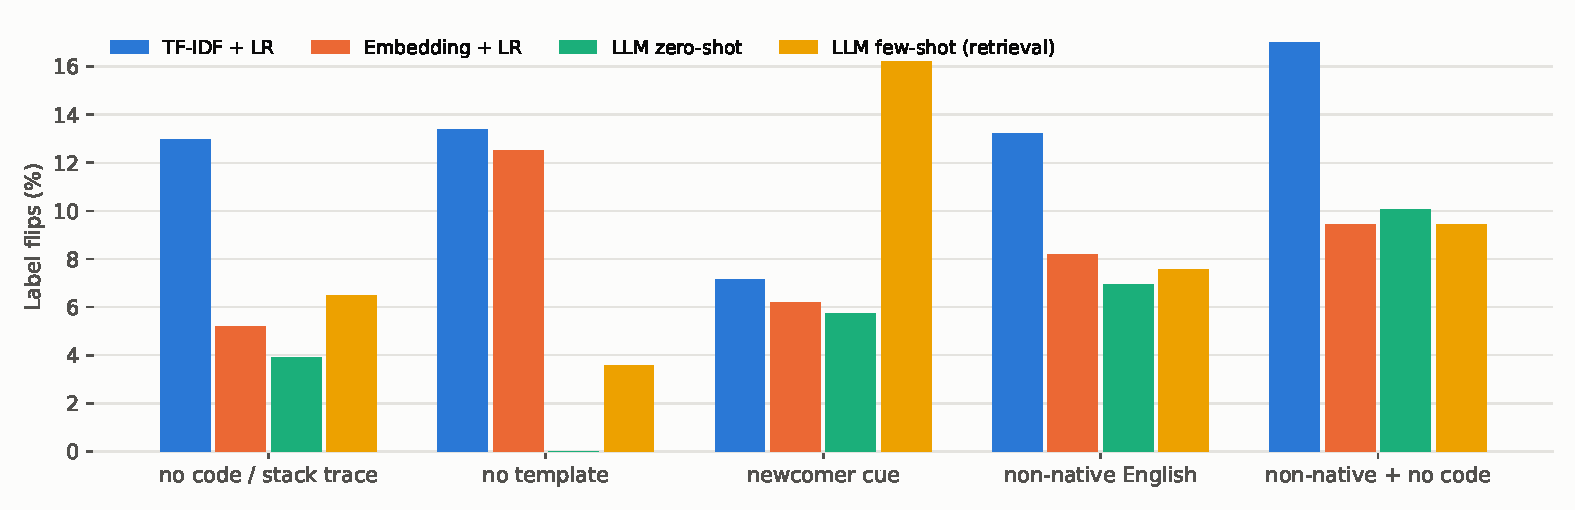
\includegraphics[width=\columnwidth]{flips.pdf}
\caption{Label flips under rewording.}\label{fig:flips}
\end{figure}

\subsection{RQ4: Are the explanations faithful?}
Asked for a label and two exact quotes as evidence, the few-shot LLM quoted the issue in 178 of 210
cases; 93.1\% of its 331 quotes occur verbatim, and the explained label matches the scored label in
92.9\% of issues. Faithfulness is weaker. On 164 issues with locatable quotes (on average 130 of 921
body characters), deleting the quoted evidence lowered the calibrated probability of the predicted
label by 0.025, against 0.014 for deleting random text of the same length (Wilcoxon $p{=}0.115$); it
changed the label in 6.1\% of issues against 3.0\% for random deletion, and lowered confidence more than
random deletion in only 55.5\% of issues. The quotes are plausible and real, but the decision is spread
across the issue and the retrieved examples; they should not be presented as \emph{the} reason.

\subsection{RQ5: Which signal notices a changed stream?}\label{sec:monitor}
We simulate 300 streams per shift: 400 in-distribution requests, then 200 from 2025--26, from a
repository without history, or in non-native English. A signal alarms when its rate over the last 50
requests exceeds the in-distribution mean plus three standard deviations. Table~\ref{tab:mon} and
Figure~\ref{fig:mon}: \emph{novelty}, one minus the cosine similarity to the closest labeled history
issue the service may retrieve from, detects a new repository a median of 11 requests after the shift
and 2025--26 traffic after 38 (98\% of runs), with no false alarms. The model's own signals --- share
handed to a human, low confidence, disagreement with the embedding classifier --- detect these shifts
in under a third of runs, and the predicted-label distribution in at most half. No signal reliably
notices the non-native stream. Model-confidence monitoring alone would miss drift that input
monitoring catches immediately.

\begin{table}[t]
\caption{Detection delay after a shift: median requests to the first alarm (share of 300 runs
detected); --: detected in fewer than half.}\label{tab:mon}
\small
\setlength{\tabcolsep}{4pt}
\resizebox{\columnwidth}{!}{\begin{tabular}{lrrrrr}
\toprule
Shift & Handoff & Low conf. & Disagree & Novelty & Label shift \\
\midrule
2025--26 issues & -- & -- & -- & 38 (98\%) & -- \\
New repository & -- & -- & -- & 11 (100\%) & -- \\
Non-native & -- & -- & -- & -- & -- \\
\bottomrule
\end{tabular}
}
\end{table}

\begin{figure*}[t]
\centering
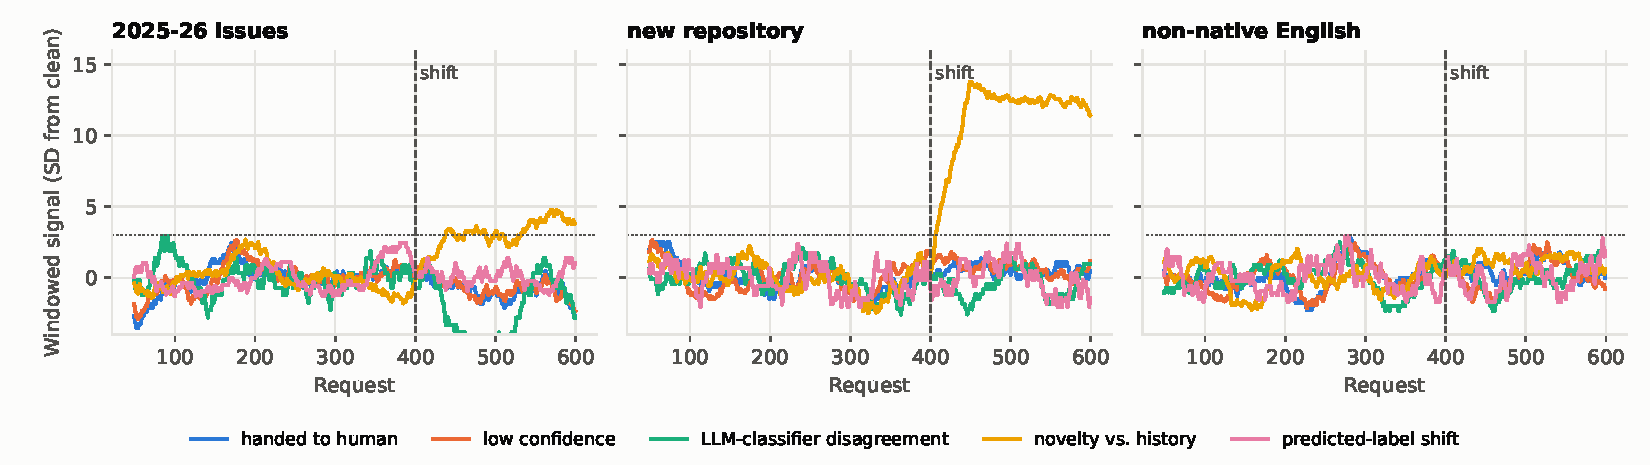
\includegraphics[width=0.92\textwidth]{monitoring.pdf}
\caption{Windowed signals in one simulated stream per shift, standardized against the clean segment;
the dotted line is the alarm level.}\label{fig:mon}
\end{figure*}

\subsection{Regression tests}
A 40-case suite (issues auto-labeled correctly, wrong predictions that must be handed off, and
rewrites that must keep their label) replays the full pipeline from recorded model scores in about 6
seconds. Injecting plausible bugs and replaying live: removing temperature scaling fails 14 cases
(every must-hand-off case is then auto-labeled), retrieving examples from other repositories fails
10, cutting the issue body to 300 characters fails 6, dropping retrieval fails 5, and removing the
label definitions from the prompt fails only 1, a gap in the suite.
